\chapter{関連研究}
\label{chapter:relatedwork}
本章では,関連研究について述べ,本研究の位置付けを明らかにする.

\section{ARを用いた情報提示に関する研究}
  \subsection{拡張現実感}
    拡張現実感(Augmented Reality; AR)とは,ユーザが見ている現実のシーンに仮想物体を重畳することで,ユーザがいる場所に応じた情報を直感的に提示する技術の総称である\cite{Kambara:2010}.近年,ARを用いたナビゲーションシステムや付加情報提示システムが多数提案されている.ARは主に,Location--based ARとVision--based ARに分類できる\cite{Chatzopoulos:2017}.

  \subsection{ARを用いたナビゲーションに関する研究}
    ARを用いたナビゲーションシステムに関する研究も行われている.
    屋外でのナビゲーションは主にLocation-based ARが用いられており,それに対して屋内でのナビゲーションは主にVision-based ARが用いられている.

    Location-based ARを用いた屋外ナビゲーションシステムの例として,図\ref{figure:arcity}に示すBlippar株式会社\footnote{\url{https://www.blippar.com}(2019/2/5存在確認)}のARCity\footnote{\url{https://itunes.apple.com/us/app/arcity-ar-navigation/id1282527727}\label{footnote:arcity}(2019/2/5存在確認)}が挙げられる.ARCityは,GPSを用いてユーザの絶対位置を特定し,ARKit\footnote{\url{https://developer.apple.com/arkit}(2019/2/5存在確認)}を用いて地形を認識することで,目的地までの道のりを示す矢印をスマートフォンの画面に重畳表示している.
    しかし,このようなLocation-based ARを用いたシステムは,地図上での目的地に到着した後,ユーザが現実世界上で目的地を探す必要がある.
    \begin{figure}[tb]
      \centerline{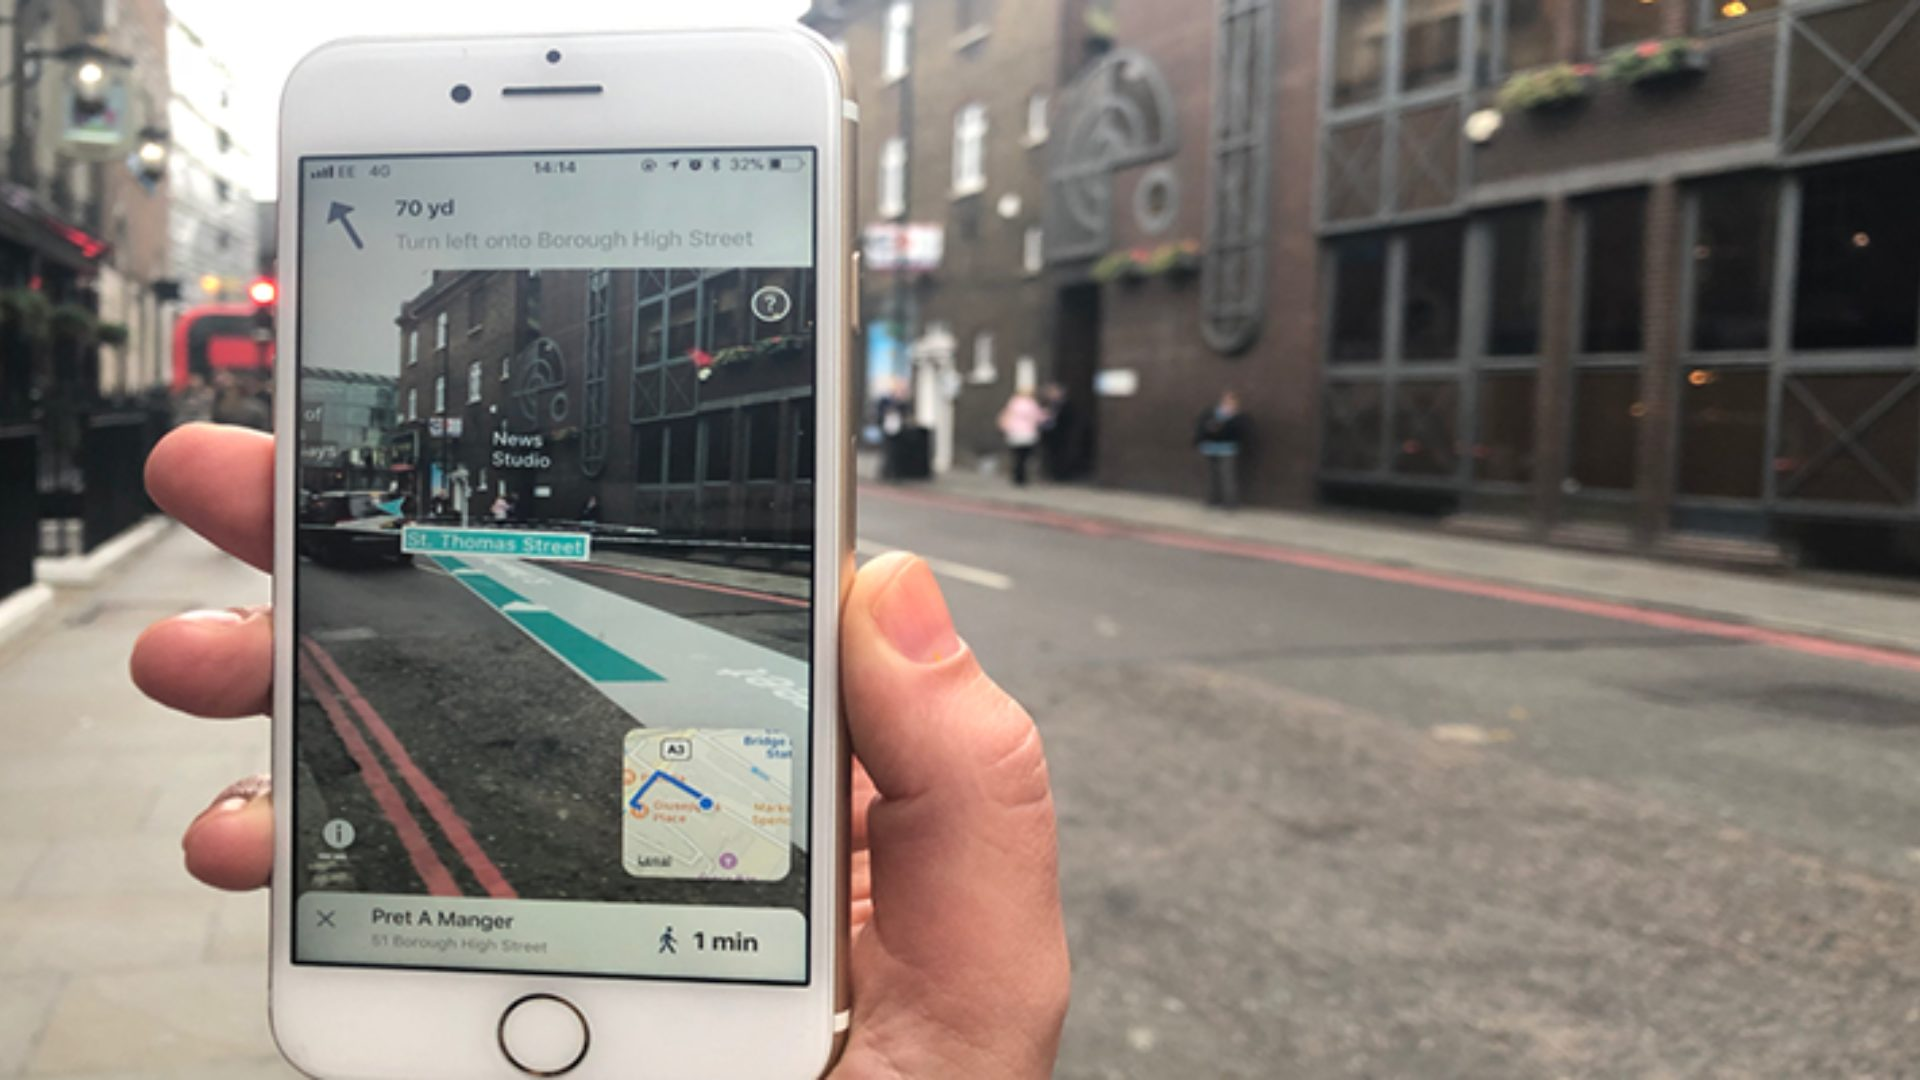
\includegraphics[width=\columnwidth, clip]{arcity.jpg}}
      \caption{ARCity(脚注\ref{footnote:arcity}より図引用)}
      \label{figure:arcity}
    \end{figure}

    Vision--based ARはさらにMarker-based ARとMarkerless ARに分類できる\cite{Rabbi:2013}.
    Marker-based ARを用いた屋内ナビゲーションシステムの例として,吉野らは,迷いやすい人の特徴を考慮した上で,QRコードマーカを目印とし,スマートフォン画面上にARで進むべき方向の矢印を表示する屋内ナビゲーションシステム``DoCoKa''を開発している\cite{Yoshino:2013}.
    Kochらは,出口の案内板など自然なオブジェクトをARマーカとしたナビゲーションシステムを開発している\cite{Koch:2014}.これにより,屋内において煙が探知された際に,作動した煙探知機までの経路を提示し,ARを用いて対処方法を提示している.
    \begin{figure}[tb]
      \centerline{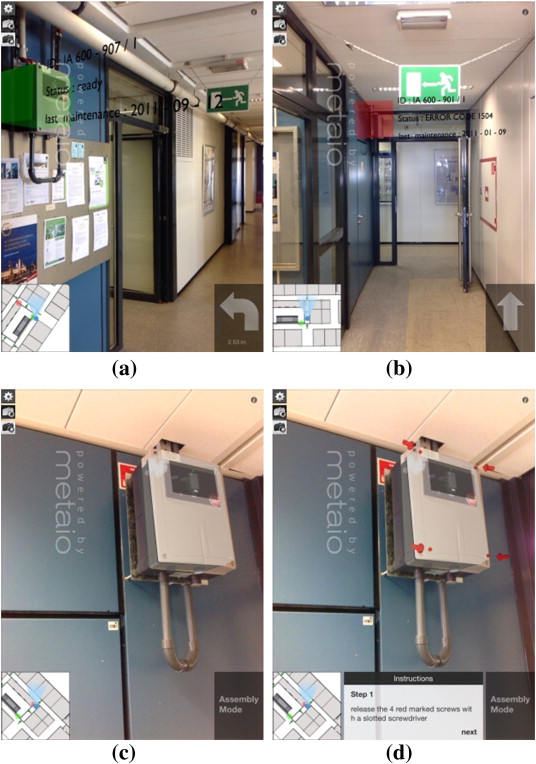
\includegraphics[width=\columnwidth, clip]{koch.png}}
      \caption{Marker-based ARを用いた屋内ナビゲーションの例(文献\cite{Koch:2014}より図引用)}
      \label{figure:koch}
    \end{figure}

    Markerless ARを用いた屋内ナビゲーションシステムの研究も行われている.
    Rehmanらは,ウェアラブルデバイスであるGoogle Glass\footnote{\url{https://x.company/glass}(2019/2/7存在確認)}を用いて,図\ref{figure:rehman}のように屋内の構造を3次元のポイントクラウドとすることにより,搭載されているカメラでポイントをトラッキングしてナビゲーションを行うシステムを提案している\cite{Rehman:2015}.
    \begin{figure}[tb]
      \centerline{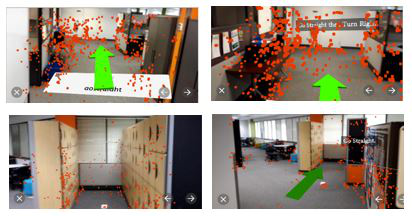
\includegraphics[width=\columnwidth, clip]{rehman.png}}
      \caption{Markerless ARを用いた屋内ナビゲーションの例(文献\cite{Rehman:2015}より図引用)}
      \label{figure:rehman}
    \end{figure}
    岩名地らは,ウェアラブルデバイスであるSmartEyeglass\footnote{\url{https://developer.sony.com/ja/develop/smarteyeglass-sed-e1}(2019/2/7存在確認)}のジャイロセンサを用いて,歩行者の視点情報に対応した案内情報を生成し,ユーザに提示するシステムを提案している\cite{Iwanaji:2016}.
    Gerstweilerらは,RGB-Dカメラを用いて屋内環境を6自由度でトラッキングし,目的地までの最短経路を算出するアルゴリズムを提案している\cite{Gerstweiler:2018}.

    しかし,これらのVision-based ARのみを用いたシステムは,屋内など特定の場所でしか利用できない.
    
    このような携帯端末上でのARを用いたナビゲーションは,紙の地図を用いた場合と比較して,より短い時間と少ない操作で目的地まで辿り着けることが明らかとなっている\cite{Rehman:2017, Yoshino:2013}.
    

\section{情報の視認性に関する研究}
  畑らは,画像内に高解像度領域と低解像度領域を作ることによって,ユーザに気づかせることなく視線を特定の領域に誘導させる手法を提案している\cite{Hata:2016}.
  例として,図\ref{figure:hata} --(a)に示す画像をユーザに提示すると,ユーザの視線がどこに集中しているかを示すヒートマップは図\ref{figure:hata} --(b)のようになる.
  \begin{figure}[tb]
    \begin{minipage}{0.49\hsize}
      \begin{center}
        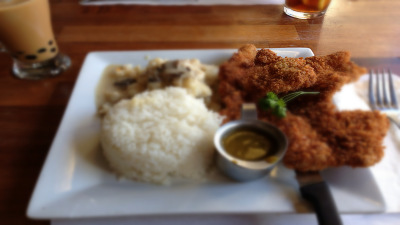
\includegraphics[clip, width=\textwidth]{hata1.png}\\
        \small{(a)提示画像}
      \end{center}
    \end{minipage}
    \begin{minipage}{0.49\hsize}
      \begin{center}
        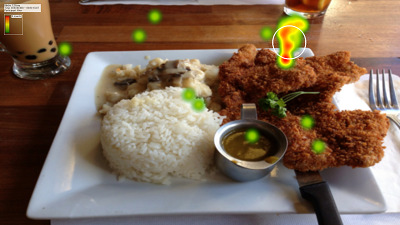
\includegraphics[clip, width=\textwidth]{hata2.png}\\
        \small{(b)ヒートマップ}
      \end{center}
    \end{minipage}
    \vspace{2pt}
    \caption{解像度制御による視線誘導(文献\cite{Hata:2016}より図引用)}
    \label{figure:hata}
  \end{figure}

  拡張現実感とは対称に,隠消現実感(Diminished Reality; DR)の研究が行われている\cite{Mori:2017}.
  DRとは,実世界から図\ref{figure:mori} --(a)のように色情報を取り除いたり,図\ref{figure:mori} --(b)のように物体を透視したり,図\ref{figure:mori} --(c)のように特定の物体を置き換えたり,図\ref{figure:mori} --(d)のように特定の物体を消去したりする技術の総称である.
  DRは主に,屋内外環境の景観シミュレーションなどに用いられている\cite{Kawai:2016}.
  \begin{figure}[tb]
    \centerline{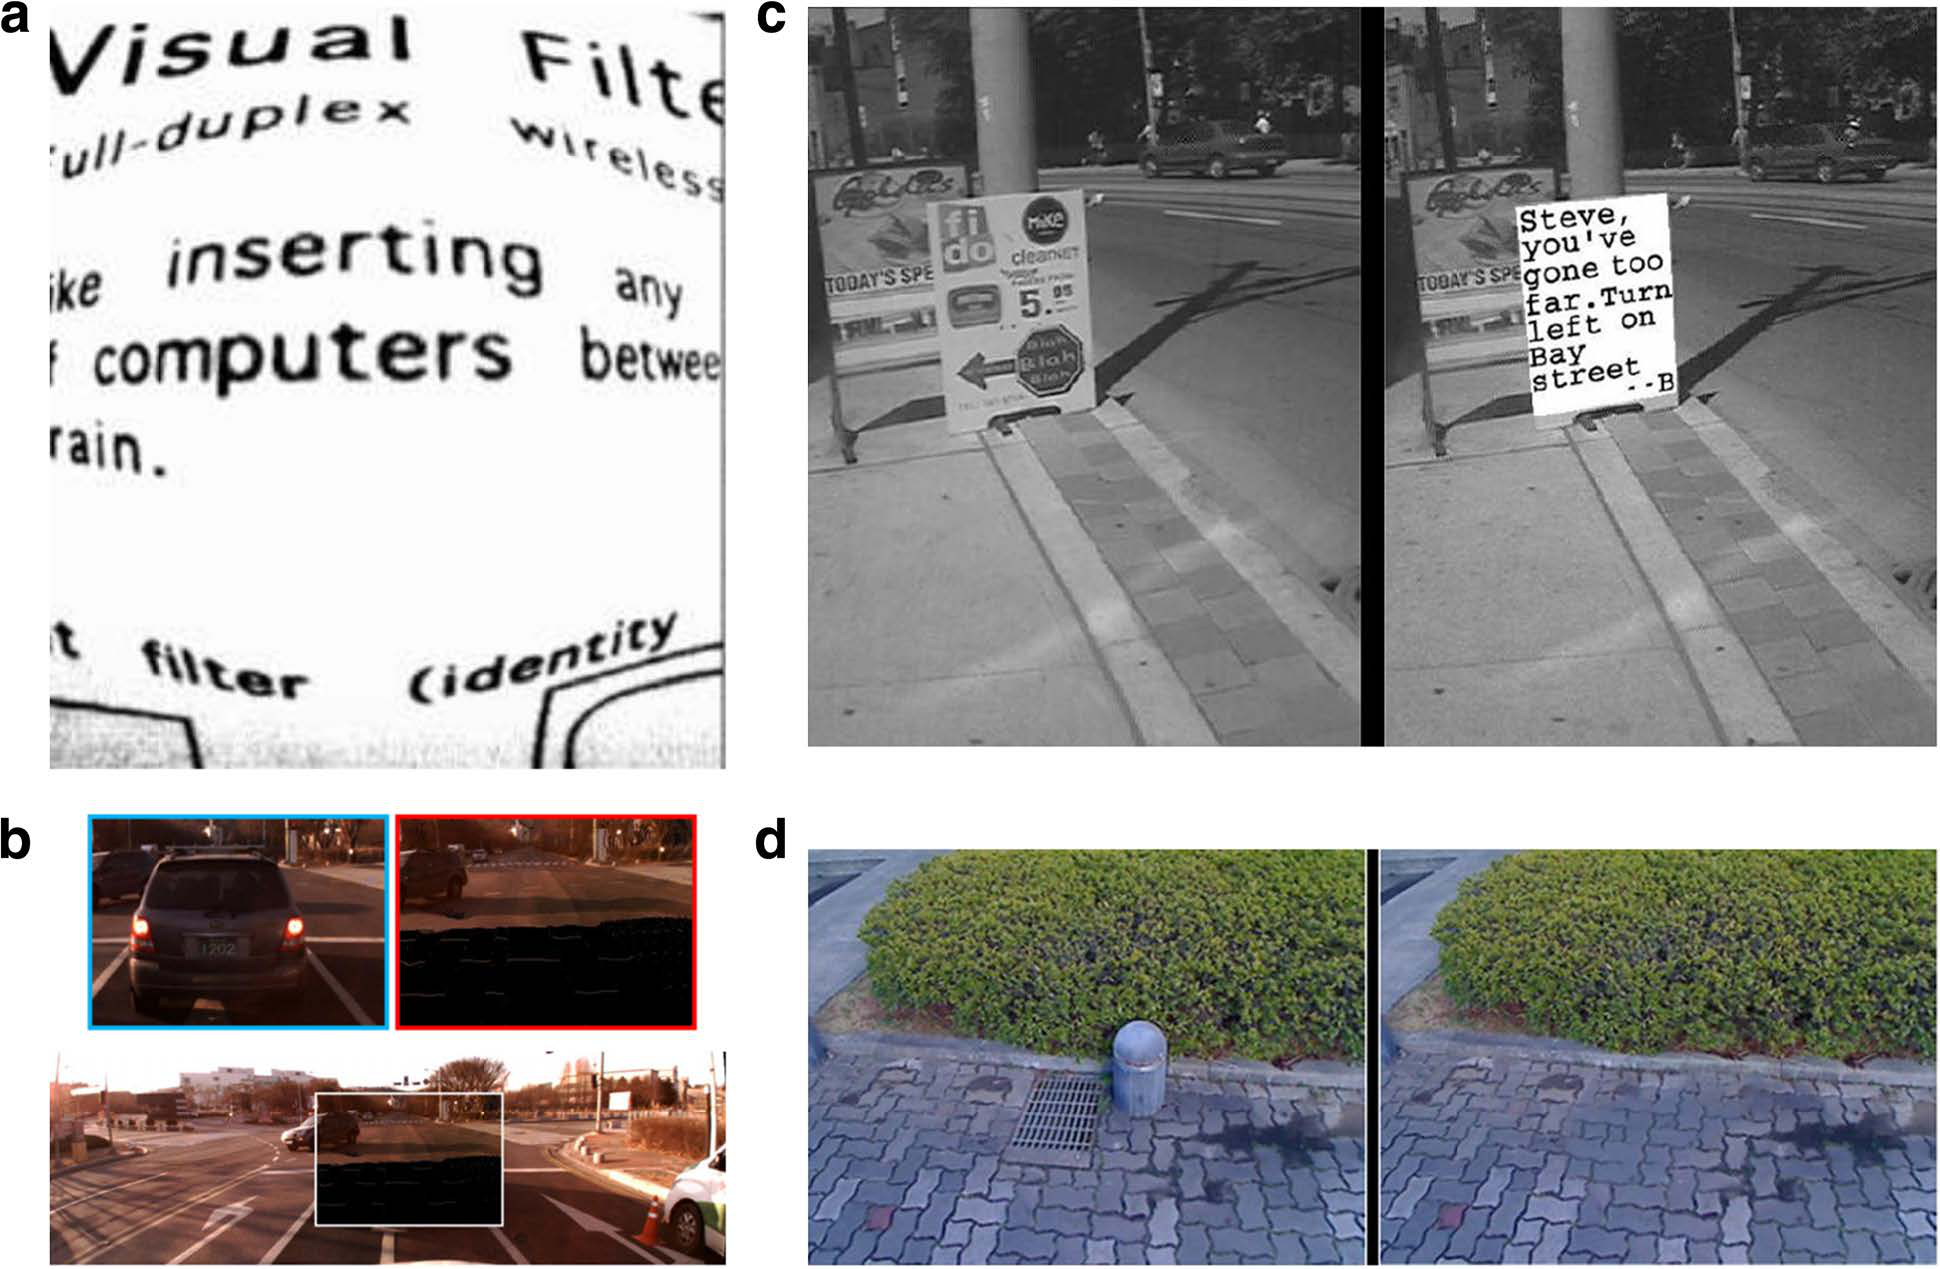
\includegraphics[width=\columnwidth, clip]{mori.png}}
    \caption{隠消現実感(文献\cite{Mori:2017}より図引用)}
    \label{figure:mori}
  \end{figure}

\section{看板認識に関する研究}
  看板を認識する研究や,看板に書かれてある文字を認識する研究は多数行われている\cite{Krishna:2018, Sasaki:2014}.
  主な手法としては,ニューラルネットワークを用いて看板に書かれている文字を認識する手法や,Optical Character Recognition(OCR)を用いる手法が挙げられる.
  Heらは,シーケンスラベリング問題として背景から文字を読み取る再帰型ニューラルネットワークを開発している\cite{He:2016}.
  Kavatiらは,図\ref{figure:kavati}のようにスマートフォンで撮影された看板や標識の写真内の文字をOCRによって認識し,英語からテルグ語に翻訳してユーザに提示する旅行者向けのWebアプリケーションを開発している\cite{Kavati:2017}.
  \begin{figure}[tb]
    \begin{minipage}{0.49\hsize}
      \begin{center}
        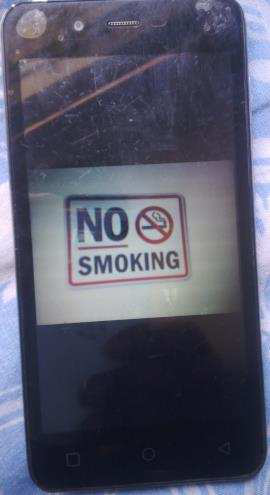
\includegraphics[clip, width=\textwidth]{kavati1.png}\\
        \small{(a)英語}
      \end{center}
    \end{minipage}
    \begin{minipage}{0.49\hsize}
      \begin{center}
        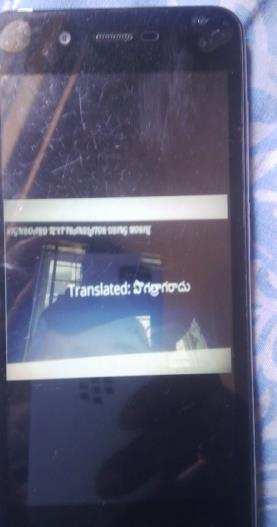
\includegraphics[clip, width=\textwidth]{kavati2.png}\\
        \small{(b)テルグ語}
      \end{center}
    \end{minipage}
    \vspace{2pt}
    \caption{翻訳された看板の文字(文献\cite{Kavati:2017}より図引用)}
    \label{figure:kavati}
  \end{figure}
  Leeらは,特徴量を用いてストリートビュー画像から看板の文字領域を検出する手法を提案し,OCRソフトウェアが文字認識することを容易にしている\cite{Lee:2016}.
  Huangらは,畳み込みニューラルネットワークを用いて看板の文字を認識し,店舗を識別する手法を提案している\cite{Huang:2017}.
  しかし,看板の中には図\ref{figure:he}のように手書き文字など崩した文字で書かれているものもあり,人間であっても読むことが容易でない場合がある.このような場合は,OCRを用いて文字を認識することは困難である.
  \begin{figure}[tb]
    \centerline{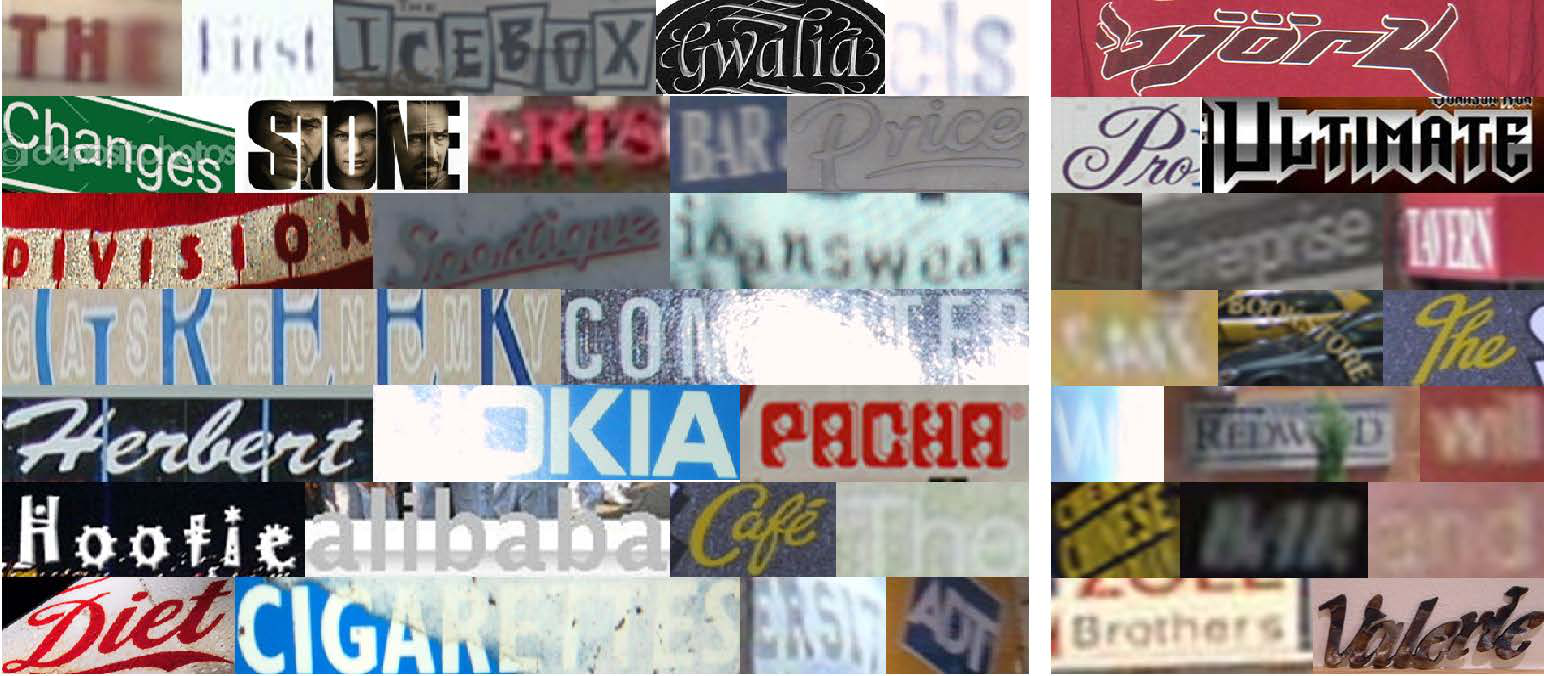
\includegraphics[width=\columnwidth, clip]{he.png}}
    \caption{文字認識が困難な看板の例(文献\cite{He:2016}より図引用)}
    \label{figure:he}
  \end{figure}
  
\section{物体検出に関する研究}
  物体検出においては,画像全体から特徴量を抽出できる畳み込みニューラルネットワーク(CNN)\cite{Lecun:1998}をベースとしたR-CNN\cite{Girshick:2014}を用いる手法が現在の主流である\cite{Nakayama:2015}.
  R-CNNでは,前処理として画像の中から物体の候補領域を予め多数取り出し,各候補領域についてCNNで物体の有無を識別することで検出を行っている.最新の手法では,図\ref{figure:ren}のように物体候補領域の生成から識別・矩形抽出までend-to-endで学習が行えるようになっている\cite{Redmon:2017, Ren:2017}.
  \begin{figure}[tb]
    \centerline{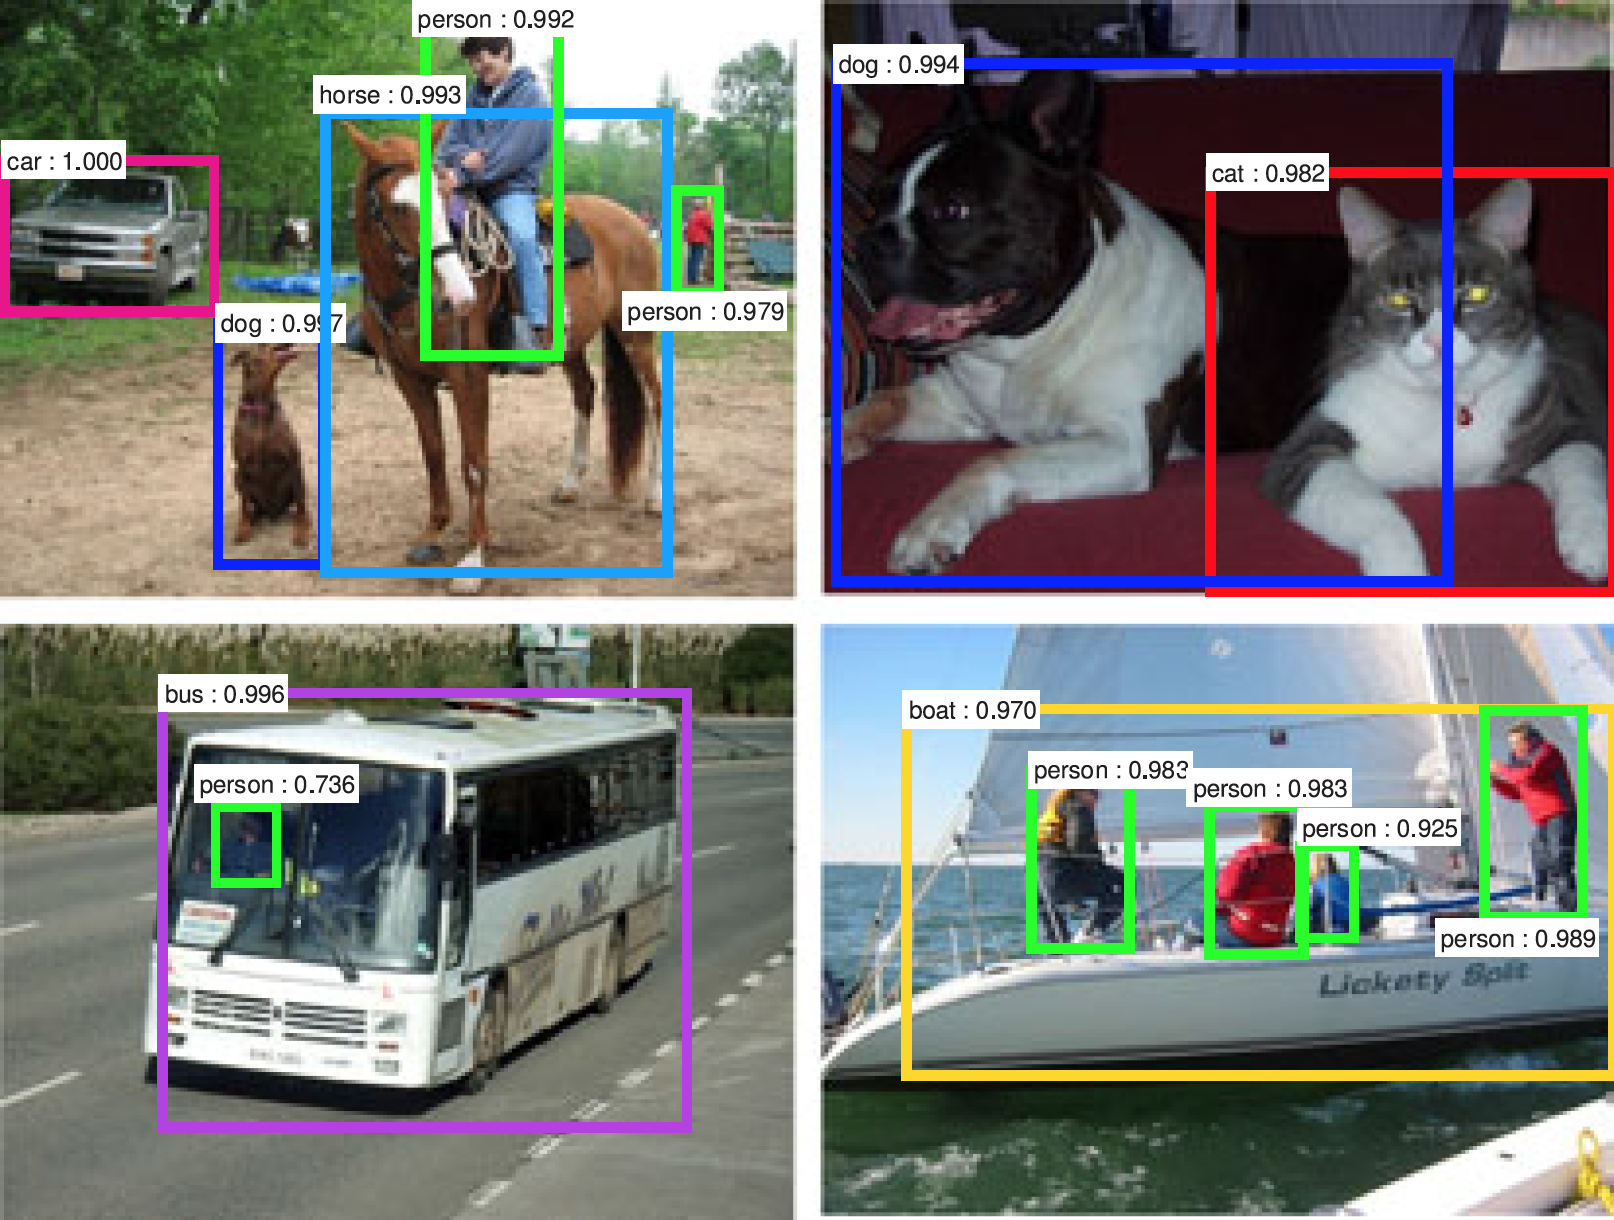
\includegraphics[width=\columnwidth, clip]{ren.png}}
    \caption{Faster R-CNNによる物体検出の例(文献\cite{Ren:2017}より図引用)}
    \label{figure:ren}
  \end{figure}

  CNNを用いた活用方法として,ImageNet\cite{Deng:2009}などの大規模教師付き画像データセットを用いた学習済みモデルが公開されている.
  このような学習済みモデルを初期値に利用し,重みデータを変更せずに特徴量抽出機として利用する転移学習や,重みデータを一部再学習して特徴量抽出機として利用するFine-Tuningを用いることによって,少ない画像データから良い精度で画像のクラス分類や物体検出ができる.
  Fine-Tuningを用いた例として,土井はWeb上からラーメン二郎の画像を収集し,ラーメンの画像から店舗を識別するモデルを構築している\cite{Doi:2018}.

\section{本研究の位置付け}
  本研究は携帯端末のカメラを通して見た画像の中から店舗を識別し,情報を重畳表示するため,Vision-based ARに分類される.
  繁華街などの視覚情報が密集している地域においては,先行研究\cite{Fujita:2013}で提案されたDRのアプローチを用いて,不要な視覚情報を目立たなくさせることによって視認性を向上させる.
  看板領域の検出には,CNNを用いたアルゴリズムであるYOLO\cite{Redmon:2017}を用い,看板画像のクラス分類にはVGG16\cite{Simonyan:2015}を用いる.